%% LaTeX2e class for student theses
%% sections/content.tex
%% 
%% Karlsruhe Institute of Technology
%% Institute for Program Structures and Data Organization
%% Chair for Software Design and Quality (SDQ)
%%
%% Dr.-Ing. Erik Burger
%% burger@kit.edu
%%
%% Version 1.3.3, 2018-04-17

% TODO find a better title for this chapter
\chapter{Applying RDF2Graph to Wikidata}
\label{ch:RDF2Graph+Wikidata}

% TODO find a better title for this section
\section{General RDF2Graph Updates}
\label{sec:RDF2Graph+Wikidata:updates}

The \branchname{master} branch of the RDF2Graph source code repository
has not seen any updates since 2015 (when \cite{vanDam2015} was published), % TODO is in-sentence \cite{} like that okay?
% TODO a) check phrasing – it’s not my intention to “call out” the RDF2Graph authors or anything :)
% TODO b) the dev branch did see some updates, I just wasn’t aware of that when I started working :/
so some updates were needed to make the program run on newer software versions
and to target a more recent version of \gls{shex}.
Many of these were rather minor in nature,
but a few of the major ones are described in this section.

The final step of the ShEx export was mostly rewritten from scratch.
This is the step that translates a JSON-LD file describing the shapes of the schema
into a ShExC file;
the previous version did this using Jade,
a templating engine for HTML documents (renamed to Pug in 2016),
constructing an HTML document containing a single plain-text \lstinline[language=html]{<pre>} element,
then extracting this text from the document using an HTML-to-text converter.
The new version directly produces the text from JavaScript
and includes several improvements:
datatypes are now properly supported,
whereas the previous version only supported a handful of hard-coded URIs as datatypes
and exported all other datatypes as if they were actually shapes;
prefixes are used everywhere in the output, highly improving readability;
and the output is sorted, making the whole generation process more deterministic
and thus making it easier to compare the results of multiple inference processes.

% TODO updates to ShEx v2 syntax – worth mentioning?
% TODO if the ShEx exporter rewrite is the only thing worth mentioning,
% the first paragraph needs to be rephrased a little,
% and perhaps the final sentence of the second paragraph can also be split up into multiple sentences

% TODO find a better title for this section
\section{Wikidata Support}
\label{sec:RDF2Graph+Wikidata:Wikidata}

The most fundamental change to make RDF2Graph support Wikidata
was % TODO is?
to change the type predicates used.
RDF2Graph heavily relies on the type information of the RDF graph it inspects,
assuming a one-to-one mapping between classes and shapes,
and it uses the standard predicates \PName{rdf:type} and \PName{rdfs:subClassOf}
to determine the class of a subject and the superclasses of a class, respectively.
However, Wikidata does not use these standard predicates:
the class(es) and superclass(es) of an item
are regular statements like any other Wikidata statement,
using the properties \PL{P31}{instance of} and \PL{P279}{subclass of}.
In the \gls{rdf} export, \PName{rdf:type} and \PName{rdfs:subClassOf} are only used
as part of the meta-model, % TODO meta-model? hm
assigning each item the class \PName{wikibase:Item}, a subclass of \PName{wikibase:Entity}.
To use the type information within the data instead of this meta-model,
RDF2Graph was changed to use the predicates \PName{wdt:P31} and \PName{wdt:P279} % TODO we haven’t seen the wdt: syntax yet, should that be in the Background?
instead of \PName{rdf:type} and \PName{rdfs:subClassOf}.

Another important aspect is that it’s not feasible to run RDF2Graph on the entirety of Wikidata at once.
For example, the 2018-08-20 full Wikidata dump is \SI{42.7}{\giga\byte} large after gzip compression % TODO >300GB uncompressed (309657344438 bytes), which is probably more impressive
and \num{8316156305} lines long uncompressed,
with most lines corresponding to one triple (except for some blank lines).
More importantly, inferring a single schema from all of Wikidata is also not the intention of this work:
the intention is to infer a schema from a particular set of exemplary items, % TODO awkward passive voice (“*the* intention” is *my* intention, I guess)
and ignore similar items which are not as exemplary (e.~g. not as well maintained)
as well as unrelated items. % TODO that should be explained in more detail in the Introduction, which I haven’t written yet as of this writing
So instead of running RDR2Graph directly against the SPARQL endpoint of the Wikidata Query Service,
a process was set up % TODO super awkward passive voice
to download the data of all selected items as well as the items they directly link to,
load that into a single N-Triples file,
serve that file via a local Fuseki SPARQL server,
run RDF2Graph against that server,
and finally run the ShEx exporter against RDF2Graph’s results.
To make it easier to run, the entire process is controlled by a Makefile in the RDF2Graph repository,
so that after creating a \filename{\variable{example}.entities.sparql} file with a SPARQL query selecting the exemplary items,
it is sufficient to run \command{make \variable{example}.shex} to run the entire process and generate the ShEx file.

This data download step also presents a convenient opportunity to drop some data from the items.
For one, the labels, descriptions and aliases of an item can make up a large portion of its data,
but are generally not interesting for ShEx schemas,
since there is rarely more to say about them than
“an item has one or more labels, zero or more descriptions, and zero or more aliases”. % TODO express as ShExC?
% TODO in theory it’s possible for items to have zero labels…
(A manually curated schema might go beyond this –
perhaps requiring, for example, that items about Spanish municipalities have a label in Spanish –
but such details are beyond the ability of RDF2Graph to infer.)
Additionally, Wikidata items often have a number of statements listing external identifiers for the item
(that is, identifiers in other databases for the same concept described by this item):
for example, Wikidata’s \Q{Q80} corresponds to \loc{no99010609} in the \gls{loc},
\viaf{85312226} in the \gls{viaf},
\imdbName{nm3805083} in the \gls{imdb},
\TwitterAccount{timberners\_lee} on Twitter,
and dozens of other external identifiers. % TODO is a vague “dozens” okay?
All these external identifiers are technically just ordinary statements,
but since they are generally not very interesting compared to other statements,
they are sorted into a separate section when viewing the item on the Wikidata website.
To reduce the runtime of the RDF2Graph inference process,
and to reduce clutter in the inferred schemas,
the labels, descriptions, aliases, and external identifiers of an item
are therefore excluded when downloading the data for a set of exemplary items.

However, one unfortunate consequence of running RDF2Graph against a reduced data set
is that RDF2Graph cannot see the full type hierarchy of the classes involved:
for example, depending on how much data was downloaded,
it may or may not be aware that the classes \QL{Q112099}{island nation} and \QL{Q3624078}{sovereign state}
have a common superclass, \QL{Q7275}{state},
which reduces the available options during the simplification step. % TODO not happy with this phrasing
To mitigate this, RDF2Graph was patched % TODO awkward passive voice
to allow specifying an alternative SPARQL endpoint for all queries that require a full view of the data,
and uses this alternative endpoint for the query to get all parent and child classes of a class.
The Makefile-controlled process mentioned above % TODO awkward phrasing
specifies the Wikidata Query Service SPARQL endpoint for this option,
so that RDF2Graph can learn the full class hierarchy around all relevant items % TODO is “learn” the right word?
even when running against a subset of Wikidata. % TODO “subset of Wikidata”? not quite happy with that phrasing

The simplification process also required some changes to support Wikidata.
Originally, RDF2Graph would merge all classes into their superclass,
almost completely unconditionally,
stopping only at the root class \PName{owl:Thing}.
This was much too aggressive for Wikidata:
not only does Wikidata have a different root class (\QL{Q35120}{entity}),
but it also has a complex hierarchy of abstract classes below that root class,
and merging other classes into those abstract classes
(like \QL{Q151885}{concept}, \QL{Q7184903}{abstract object} or \QL{Q830077}{subject})
would not result in useful schemas.
Therefore, the merging step in the simplification process was adapted % TODO awkward passive voice
to add a number of Wikidata items to the set of classes which other classes should not be merged into
(originally only containing \PName{owl:Thing}),
and to stop looking for common superclasses of two classes after checking five levels in the class hierarchy.
(The limit of five levels is an arbitrary choice
and could also be made configurable if deemed necessary in the future.) % TODO look a bit more into this?
% TODO also disabled step 7.4.4 (dropping predicates that were found in superclasses)
% because the superclass support in the ShEx export changed,
% but that requires explanation of how the ShEx export changed

% TODO find a better title for this section
\section{Support for cyclic graphs}
\label{sec:RDF2Graph+Wikidata:cyclic-graphs}
% TODO this whole section mixes parent/child and parent class / subclass terminology :/

As outlined in \cref{sec:Background:RDF2Graph}, % TODO style?
RDF2Graph has an optional simplification feature
where the schema will be simplified in several steps,
based on the type hierarchy of the classes involved.
For this, the type hierarchy is loaded into an in-memory data structure,
which in the code is referred to as a \emph{tree}. % TODO is the emphasis here appropriate? feels odd
In fact, the data structure forms a generic, directed graph,
where each node may have any number of children and any number of parents,
and no restrictions on the structure are enforced during construction.
However, while the algorithms subsequently operating on the data structure support classes with multiple parent classes,
they do assume that the graph is acyclic,
i.~e., that no class is an indirect subclass of itself.

This assumption makes sense in general,
since a type hierarchy is usually assumed to be acyclic:
if there is a cycle in the subclass relations between a list of classes,
that effectively renders all these classes equivalent,
since any instance of any one of these classes is then also an (indirect) instance of all other classes.
However, experience shows % TODO “experience shows” sounds extremely dodgy
that occasional emergence of subclass cycles is almost unavoidable on Wikidata:
any one of the subclass links may appear reasonable for just the two items it connects,
and an editor looking at these items will not necessarily notice that a cycle has been formed,
since the other statements forming the cycle are not visible when looking at these two items.
These cycles are eventually found and fixed by the community,
but in the meantime, it’s possible that RDF2Graph will run on a subclass graph containing cycles.
% TODO example? https://www.wikidata.org/wiki/Special:Diff/735108434
Therefore, to make the process more robust, % TODO “the process” is probably a weasel word here
several algorithms in the simplification step were adjusted to be able to cope with cyclic graphs.
% TODO explain why we even bother with this:
% though the results *in the cycle* may be nonsensical, the rest of the schema should not be affected

A general component of the new algorithms are methods to get all children and parents of a node,
in a matter that is guaranteed to terminate even if there are cycles among the children or parents.
The method for collecting all child nodes is outlined in \cref{alg:GetAllChildren},
and the method for collecting all parent nodes is completely analogous.
Since each node can only enter the return set once,
the queue only grows when nodes are added to the return set,
and each iteration takes one node from the queue,
the algorithm must eventually exhaust the queue and terminate,
provided that the set of nodes reachable from the initial node is finite.
% TODO should this be a more formal proof?

% TODO it feels highly unlikely that this algorithm doesn’t have some existing name
\begin{algorithm}
  \begin{algorithmic}
    \Function{GetAllChildren}{node}
    \State $\Instruction{initialize \Variable{set} of all children (empty)}$
    \State $\Instruction{initialize working \Variable{queue} of children (empty)}$
    \State $\Instruction{add to \Variable{queue}} \gets \Instruction{direct children of \Variable{node}}$
    \While{$\Variable{queue} \neq \emptyset$}
    \State $\Variable{child} \gets \Instruction{take from \Variable{queue}}$
    \If{$\Variable{child} \not\in \Variable{set}$}
    \State $\Instruction{add to \Variable{set}} \gets \Variable{child}$
    \State $\Instruction{add to \Variable{queue}} \gets \Instruction{direct children of \Variable{child}}$
    \EndIf
    \EndWhile
    \State \Return $\Instruction{\Variable{set}}$
    \EndFunction
  \end{algorithmic}
  \caption{An algorithm to collect all direct and indirect child nodes in a graph.}
  \label{alg:GetAllChildren}
\end{algorithm}

With this in place,
it becomes easy to reimplement the method which counts the number of direct and indirect instances of each class,
based on the direct instance counts on each class node.
Previously, the method operated recursively,
aggregating instance counts for each indirect subclass of a class
all the way up to the class itself,
and this recursion would never terminate when encountering a cycle of subclasses.
Instead, the new implementation collects all direct and indirect subclasses up-front using \cref{alg:GetAllChildren}
and then sums up their direct instance counts.

Two steps of the simplification process % TODO give the step numbers in the Introduction and reference them here
remove some of the temporary (added) type links of a node,
based on the temporary type links of its neighboring node:
one step removes temporary type links from parent classes that are only found in one child class,
the other removes temporary type links from child classes that are made redundant by a type link in the parent class.
Both steps were originally implemented as inspecting the neighboring nodes’ temporary type links
and then directly manipulating the node’s own temporary type links.
This required that each step traversed the nodes in the correct order
(parents before children for the first step,
children before parents for the second step)
and was implemented by traversing the graph recursively,
which is problematic if the graph contains cycles.
% TODO all this anonymous steps and parts business sounds clumsy
% give all of them numbers and/or names and then rephrase this
This problem was solved by splitting up the analysis and modification of the temporary type links:
each step now has two parts,
where the first part marks all temporary type links that should be removed,
and the second part actually removes them from a node’s temporary type links.
As long as the first part for all nodes is run before the second part for any node,
these parts can now be run in any order,
and instead of recursively traversing the graph,
both steps now first collect all child nodes of the root node
and then iterate them twice,
running the first part the first time and the second part the second time.
% TODO pseudocode algorithms for any of this paragraph?

RDF2Graph also has a method to determine the distance of all indirect parents from a certain node,
which is used when searching for common superclasses of a class.
Like the other methods, this was implemented recursively,
setting the distance of a parent node to the current value of a counter
and then calling the same method on all parent nodes of that node with the counter incremented by one.
In this case, the recursion was kept,
but the method was adjusted to only visit a parent node
if it has not been visited before, or if its current distance is larger than the counter value.
The second part of the condition is necessary to ensure that the distance is set correctly
if a node is visited first via a longer path and then later again via a shorter path,
which is possible since the method implements a depth-first search instead of a breadth-first search.
(In fact, the previous implementation had a bug here,
where the distance would be incorrect if a node was visited first via a shorter path and then later again via a longer path,
since it would always unconditionally override the distance.)
% TODO pseudocode for this?

% TODO perhaps just drop this paragraph? it’s really trivial
And finally, there is also a method to determine whether a certain node is a (direct or indirect) parent node of another node.
This was originally implemented recursively,
% TODO phrasing here feels convoluted
but could be replaced with a simple check whether the potential parent node is an element of the set of the child node’s parent nodes,
using \cref{alg:GetAllChildren}.

% TODO find a better title for this section
\section{Schema Reduction}
\label{sec:RDF2Graph+Wikidata:schema-reduction}

An unexpected problem emerged once the schema inference itself was in place: % TODO phrasing: “in place”?
it proved to be almost impossible to validate items against the inferred schemas
for all but the most simple data sets.
Two ShEx implementations were evaluated:
shex.js, % TODO link? cite?
a JavaScript implementation running in Node.js,
and shex-java,
a Java implementation offering two different validation algorithms \cite{boneva:hal-01590350}.
shex.js would usually crash with an out-of-memory error from Node.js within a few minutes,
whereas shex-java would run for hours on end without any output or apparent progress
(with either algorithm).

One attempted strategy to be able to validate the inferred schemas % TODO “attempted strategy”? feels awkward
was to reduce the size of the schemas by dropping some less-relevant elements.
This was part of the motivation for dropping labels, descriptions, aliases, and external identifiers of an item
from the data set that the inference would be run against
(see \cref{sec:RDF2Graph+Wikidata:Wikidata});
however, reducing the input data set is not the only way to reduce the resulting schema:
it is also possible to further trim the schema after the inference process has finished.
This was implemented in the final step of the ShEx exporter, % TODO mention shexbuilder.js file name?
which had already been mostly rewritten for different reasons
(see \cref{sec:RDF2Graph+Wikidata:updates}).
RDF2Graph tracks the number of instances of each class it encounters,
and this information is still available to the ShEx exporter,
which makes it possible to decide which elements of a schema to keep and which to drop
based on how often those elements were used in the original data. % TODO add example?

% TODO somewhere around here we need to explain why it’s okay to drop elements.
% type links → our schemas aren’t perfect anyways; predicates → shapes are not closed; shapes → unused
% (does “open world” vs. “closed world” factor into this?)

Elements can be removed from a schema on three different levels:
an individual type link can be removed from a predicate, % TODO probably needs explanation
a predicate can be removed from a shape,
or an entire shape can be removed from the schema.
Removal on the first two levels can be decided for each element independently,
but whether a shape can be removed from the schema depends not only on how many instances of that shape exist,
but also whether the shape is referred to by any type links that were not dropped from this schema.
To avoid dropping shapes which are needed by other parts of the schema,
while still dropping shapes that are otherwise unused,
the exporter maintains two sets of shapes:
one for shapes which are referenced from type links,
and one for shapes which may be dropped.
When printing the final schema, only shapes found in the latter set but not in the former are skipped.

The decision whether to drop an element or not
was implemented as a simple numeric threshold on all three levels:
if a type link is used less than $m$ times, % TODO verify this: is the “count” of a typelink really the number of times it occurs?
a predicate is used less than $n$ times (sum of all type link uses),
or a class has less than $o$ instances,
the element is dropped.
The three limits are independent,
though in practice it makes most sense to choose them such that $m > n > o$.
% TODO does it make sense to describe this strategy here?
An alternative strategy to explore in the future might be
to turn those fixed thresholds into ratios,
so that the same parameters can be used for vastly different data sets
with varying numbers of class instances overall.

Unfortunately, this strategy was not very successful in enabling validation of the schemas.
Only at almost draconian thresholds for dropping elements,
where only a few shapes and predicates would remain in the schema,
would validation succeed;
manual bisecting of the schemas which failed to validate
would often turn up a fairly small problematic part of a schema
which a simple count-based threshold was ill-suited to detect automatically.

% TODO find a better title for this section
\section{Depth Limits in Validation}
\label{sec:RDF2Graph+Wikidata:depth-limit}

Another attempt to make validation of the inferred schemas more feasible
was to limit the maximum depth during the validation process. % TODO better word than “process”?
Consider, for example, a simple shape for humans, % TODO only prose or also ShExC?
which describes a human as having any number of human parents and a date of birth.
To validate whether any given node is actually a human,
all its direct and indirect parents must also be validated,
potentially thousands of ancestors, no matter how remote.
If the shape is more complicated,
with more predicates potentially linking to other shapes as well,
this can get very expensive rather quickly.
On the other hand, it is not clear that the more remote validations here are useful,
at least in the context of validating Wikidata items
(where different areas of items may be edited by very different sets of editors)
against automatically inferred schemas
(which are likely to have inherited some imperfections from the input data): % TODO there should be a longer paragraph on this somewhere else, perhaps add a \cref once it exists
experience shows that % TODO is “experience shows” acceptable?
most inferred schemas tend to include shapes for certain core classes,
e.~g. \QL{Q5}{human} or \QL{Q3624078}{sovereign state},
but someone attempting to validate an item for a mammalian protein
is unlikely to care that the item for the protein’s discoverer’s husband’s country of citizenship % TODO too many ’s?
happens to be missing an \PL{P1279}{inflation rate} statement.

Therefore, % TODO is it okay to start a paragraph with “therefore”?
in an attempt to reduce the amount of irrelevant violations
and to make the validation terminate without crashing,
a patch to add an optional depth limit to the shex.js implementation was developed.
With this change, if the depth limit was reached,
the validator would skip recursing into another shape
and instead only record the fact that the limit was reached before continuing.
Unfortunately, however, this proved unsuccessful.
When testing some items against several inferred schemas,
low limits (2–4) would yield unpredictable results
(sometimes validate successfully, sometimes report problems, sometimes crash),
whereas higher limits (up to 10) would typically have the same result as validation without any depth limit
(either validation failure or crash),
though sometimes with wildly varying runtimes.
(More details can be found in \cref{sec:appendix:depth-limit}.)
One possible explanation for this is that pruning one part of the validation process when reaching the depth limit
may cause the validator to spend more time in other areas,
which may previously not have been necessary if the pruned part would otherwise have resulted in a violation.
% TODO I’m not sure if that makes sense

% TODO also mention the attempted depth limit in shex-java?
% I have a patch stashed away for that, but I don’t remember how it worked out,
% except that generally it didn’t help that much, I think

% TODO find a better title for this chapter
\chapter{The Wikidata ShEx Inference Tool}
\label{ch:wdsi}

% TODO all of the below probably needs to go in a \section, I’m not sure what the rules on chapter introductions are

Once the schema inference process against Wikidata was more or less settled,
it was time to begin making it available to others. % TODO is “it was time to” appropriate language?
RDF2Graph, its ShEx exporter, and the Makefile-based process around them
require several different programs and programming runtimes to be available,
which it would be unreasonable to expect every interested user to install
(not to mention that the Makefile assumes a Unix-like environment,
whereas the potential users are likely to use Windows).
Instead, a common approach in the Wikimedia universe
is to install such a program on Wikimedia Toolforge
and make it available to users via a web interface.

% TODO what tense / mood to use in this section? not sure if subjunctive mood makes sense
In this Wikimedia-hosted tool,
users would enter a SPARQL query selecting the set of exemplary items from which to infer a schema,
and the tool would download the associated data,
run RDF2Graph and the ShEx exporter,
and make the ShExC output available to the user.
The simplest process for that would be
to directly return the ShExC code in the server’s response to the user’s HTTP request,
but that is not possible:
even simple inference jobs % TODO “jobs” okay?
from a single item take at least several minutes,
and more complicated jobs % TODO “jobs” again
over several dozens of items can take multiple hours –
the connection to the user would time out long before that,
and the user might also become impatient and simply close their browser window or tab.

Instead, the inference process runs in the background,
and after submitting the SPARQL query and starting the process,
the user is redirected to a page describing the currently running job.
They can periodically reload the page,
and each time the page is loaded,
the tool checks if the background process is still running.
If the background process has finished in the meantime,
the tool collects the output,
cleans up the temporary files left behind by the process,
and finally makes the output
(primarely the ShExC code, but also debugging outputs)
available to the user.

Since this already more or less requires storing inputs and outputs persistently,
a natural extension of this scheme is to make this job page available to others,
so that not only the original submitter but also other users can inspect a running or completed job.
(The input data is entirely public data from Wikidata,
so there is no reason to restrict the visibility of the outputs.)
This facilitates easy collaboration on schemas between multiple users
and allows even casual visitors to see how the tool operates,
and what kinds of results it produces,
without having to start their own inference process.
To make each result easier to comprehend for others,
users can also submit a title, description, and/or URL for additional information
along with their SPARQL query. % TODO strictly speaking, the title isn’t optional. does that matter?

As the inference process consumes a lot of resources,
it doesn’t run directly on the same system as the web server providing the tool’s front-end.
Instead, it is submitted as a job for the Sun Grid Engine system also offered by the Toolforge environment,
where it will be run on some execution host with sufficient free resources.
To ensure that the system’s resources are not exhausted by this one tool,
the tool only allows at most two jobs to run in parallel,
and prevents users from submitting any more jobs if too many jobs are currently running,
instead asking them to try again later.
Job submission is also restricted to users with a valid Wikidata account,
authenticated via OAuth.
The identity of the submitting user is another attribute of a job,
along with its title, description, URL, and SPARQL query,
and can be seen by other users who look at the pending or finished jobs of the tool.

% TODO is this paragraph relevant?
Details of each job,
such as its title, submitting user, and submission time,
are stored in a tool-specific SQL database on the Toolforge database servers.
However, the outputs of a job
(ShExC file, standard output of the process, standard error of the process),
as well as to a lesser degree the SPARQL query forming its input,
are too large to store in a database.
Instead, they are stored directly on the file system.

% TODO find a better title for this section
\section{Toolforge Support}
\label{sec:wdsi:Toolforge}

% TODO find a better title for this section
\section{Abstract Considerations}
\label{sec:wdsi:abstract}

% TODO I suppose the current paragraphs directly below the chapter mostly cover this section,
% needs to be suitably rearranged

% TODO find a better title for this section
\section{Utilities}
\label{sec:wdsi:utilities}

To make the ShEx output more readable,
support for the ShExC syntax was added to the popular Pygments syntax highlighter. % TODO link to pull request?
If the ShEx code for a job % TODO is “a job” okay?
is requested by a browser
or some other kind of client which declares that it can accept HTML
(using HTTP content negotiation),
the tool applies the Pygments syntax highlighter to the code on-the-fly
and sends a complete HTML document containing the prettified code and associated CSS rules.
Clients which do not accept HTML documents receive the plain ShExC code instead.

The HTML document that is sent to browsers
also includes a client-side script,
which searches for Wikidata item IDs in the ShExC code,
fetches the labels of all mentioned item IDs from Wikidata,
and adds them to the document in \lstinline[language=html]{<abbr>} abbreviation elements.
It also hyperlinks each reference of a shape to its definition,
and the definition to the corresponding entity on Wikidata.
This makes it much more convenient to read the schema in the browser:
the user merely has to hover their mouse over a class to see its label instead of the item ID;
clicking on it brings the user to the shape for that class;
and clicking on the ID there brings the user to the Wikidata page for the class,
where they can further explore the related data.

A comparison of the effects of these two features
can be seen in \cref{fig:shexc-syntax-highlighting}.

% TODO revisit layout of this figure when the thesis is close to done,
% perhaps adjust the widths and/or trimming depending on how the figure fits on a page
\begin{figure}[t]
  \begin{subfigure}[t]{0.45\textwidth}
    \centering
    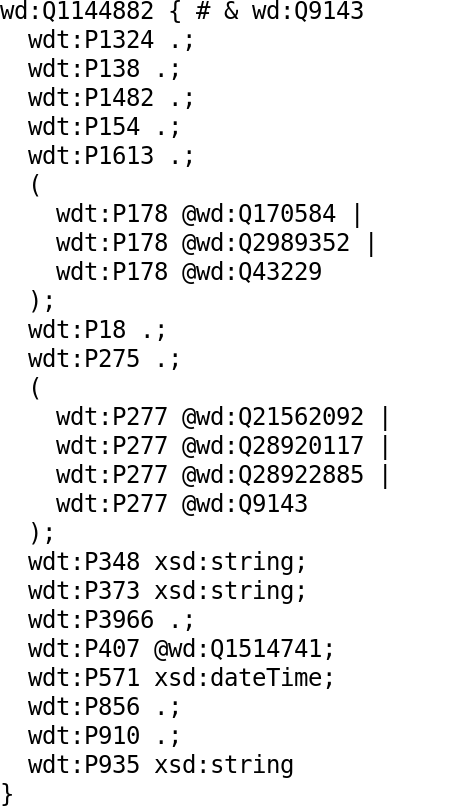
\includegraphics[trim={0 2.5cm 0 0},clip]{screenshots/shexc-no-syntax-highlighting}
    \caption{
      Excerpt of an inferred schema for Linux distributions.
    }
    \label{fig:shexc-syntax-highlighting-without}
  \end{subfigure}
  \begin{subfigure}[t]{0.45\textwidth}
    \centering
    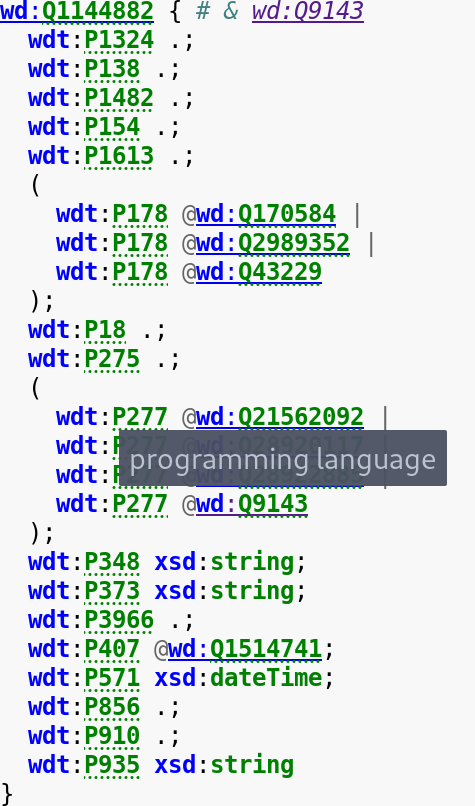
\includegraphics[trim={0 2.5cm 0 0},clip]{screenshots/shexc-with-syntax-highlighting}
    \caption{
      The same schema with syntax highlighting and the script applied.
      The cursor is over the \lstinline{P277} property ID.
    }
    \label{fig:shexc-syntax-highlighting-with}
  \end{subfigure}
  \caption{
    Comparison of the effects of syntax highlighting and the client-side script.
  }
  \label{fig:shexc-syntax-highlighting}
\end{figure}
